\documentclass[preprint]{aastex} %double-column, single-spaced document:
%\documentclass[iop,floatfix]{emulateapj} 

\usepackage{hyperref}
%\usepackage{graphicx}
%\usepackage{apjfonts}
\usepackage{enumerate}
\usepackage{amsmath,amssymb}
\usepackage{geometry}
\usepackage{bm}

\newcommand{\prob}{{\rm prob}}
\newcommand{\qN}{\{q_i\}_{i=1}^N}
\newcommand{\qM}{\{q_{im}\}_{i=1,m=0}^{N,M}}
\newcommand{\yN}{\{y_i\}_{i=1}^N}
\newcommand{\vt}{\vec{\theta}}
\newcommand{\vg}{\vt_{\star, {\rm grid}}}
\newcommand{\vstar}{\vt_{\star}}
\newcommand{\vN}{\vt_{\rm N}}
\newcommand{\vc}{\vec{c}}
\newcommand{\fM}{f_{\rm M}}
\newcommand{\fD}{f_{\rm D}}
\newcommand{\vD}{\vec{D}}
\newcommand{\dd}{\,{\rm d}}
\newcommand{\trans}{\mathsf{T}}
\newcommand{\Z}{[{\rm Fe}/{\rm H}]}
\newcommand{\A}{[\alpha/{\rm Fe}]}

%\slugcomment{}
%\shorttitle{}
%\shortauthors{}

\begin{document}

\title{A method for inference of fundamental stellar parameters using high resolution spectra}
\author{\today{}\\
\medskip
Ian~Czekala\altaffilmark{1} et al.
%Author2\altaffilmark{2},
}

\altaffiltext{1}{Harvard-Smithsonian Center for Astrophysics, 60 Garden Street MS 10, Cambridge, MA 02138}
%\altaffiltext{2}{Institution 2}
\email{iczekala@cfa.harvard.edu}

\begin{abstract}
  Matching observed spectra of stars against a grid synthetic spectra is a popular approach to determine fundamental stellar parameters such as effective temperature, surface gravity, and metallicity. However, a fundamental problem with this approach is that the synthetic spectra contain systematic errors such as wrong or missing spectral lines. In the presence of such errors, a simple $\chi^2$ fit between spectra will likely yield biased parameters and incorrect uncertainty estimates. This behaviour is analogous to the way a few strong outliers might severely bias the fit to a straight line. These spectral outliers are difficult to identify \emph{a priori}; procedures such as sigma clipping might be prone to their own systematic effects and discard useful information. We outline an approach to probabilistically identify and account for spectral features that deviate from reality. Such an approach is most needed when operating at high spectral resolution ($R >$ 10,000), since this is when systematic deviations begin to appear most striking, however our technique is still valid for lower resolution spectra as well. We also outline some approaches for spectral fits to brown dwarfs and planets, where instead of spectral lines there may be systematic deviations of a larger swath of the spectrum.
\end{abstract}

%\keywords{}

%\begin{figure}[htb]
%\begin{center}
%
\includegraphics{file}
%\caption{}
%\label{fig:}
%\end{center}
%\end{figure}

\section{Introduction and review of existing methods}

The fundamental parameters of stars---mass, luminosity, effective photospheric temperature, surface gravity, and metallicity--are of supreme interest to astrophysicists for a wide variety of reasons. A salient example is that most newly discovered exoplanets must necessarily their mass and radius measured relative to the properties of their host stars (e.g. \citealt{tfs+12,blj+12,ssm+13}) and uncertain stellar parameters translate into uncertain planet properties \citep{kan14}. The properties of stars are of course also important in their own right because they inform us about our ideas of stellar evolution \citep{dm97, bca+02}. Because stars are the fundamental units of the cosmos, techniques to infer the properties of stars date back to the dawn of astronomy. We briefly review some of the modern and popular techniques in the literature. Approaches can be broadly classified into techniques that compare stars by some broadly defined indices and techniques that attempt to forward-model an observed stellar spectrum by doing a pixel-to-pixel comparison.

\subsection{Classification techniques}
Many of existing techniques were written to analyze low to medium resolution ($R < $ 10,000) spectra. I am calling them similarity techniques because they focus on determining and recognizing patterns of spectra useful in classification.

\paragraph{Line indexes} By cataloguing the equivalent widths of chosen spectral lines into indexes, one can correlate the index with stellar properties and identify features that are sensitive temperature, surface gravity, or metallicity. Then, one matches the indecies of a new star against these relationships and derives a set of stellar parameters. A recent example using M dwarfs is \citet{nci+14}. This technique works, but there are many things that could be improved. First, the selection of which lines to measure is arduous and based upon expert knowledge of previously catalogued stars. This is both a disadvantage and an advantage. On one hand, by choosing a subset of lines to fit, one may be unwittingly throwing away useful information. On the other hand, it allows the modeller to discard regions of the spectrum that do not follow a simple trend with stellar parameters. Second, while measuring equivalent widths is easy to do, this discards any useful information contained in the shape of the line profile. 

\paragraph{Principal component analysis} PCA reduces the dimensionality of the data space and searches for the most salient features of the spectra \citep{ptb14}. How does one properly estimate parameter uncertainties in such an approach? It seems like this approach exists because it is an easy thing to do.

Matrix inversions: MATISSE \citep{rbd06}. This method is similar to PCA in that it derives basis vectors that describe the fundamental parameters of the star. In the PCA analysis, the principal components do not necessarily correspond to true physical quantities. The MATISSE algorithm determines weights that ensure the components are similar to the stellar parameters. They only test the algorithm against input synthetic stellar spectra to detect biases in the parameters, and against the Sun and Arcturus. They do acknowledge that there will be systematic deviations between the synthetic spectra and real spectra, but they do not account for the possible inflation of error estimates.

Given the inherent systematic uncertainties involved in each method, some groups elect to combine the inference from different algorithms, such as (SLOAN SSPP) \citep{lbs+08}. This approach includes machine learning along with many of the previously mentioned techniques.

\paragraph{Machine learning}
Many machine learning techniques exist and classify spectra by comparing patterns between observed spectra and a training set of spectra (which could be real spectra of stars classified by an expert or a synthetic library that has known $\vg$). However, my first impression is that these tools are designed to handle large collections of spectra from stellar surveys such as SDSS \citep{sam+10}. In our immediate project involving T Tauri stars, we only have a few ($\lesssim 20$) stars that we wish to study in exquisite detail, incorporating specific parameters such as $v \sin i$, extinction, and veiling. However, I am a novice when it comes to machine learning so I may be missing something here.

\subsection{Pixel to pixel techniques using synthetic spectral libraries}
\label{sec:pix}
Many high quality synthetic spectral grids are now available. Nearly all synthetic stellar libraries are parameterized by the ``fundamental'' stellar parameters of effective temperature, surface gravity, metallicity, and alpha enhancement. We define this combination as 
\begin{equation}
  \vg = \{T_{\rm eff}, \log(g), \Z, \A \}
\end{equation}
Naively, it makes sense to compare an observed spectrum against spectra from the synthetic grid. Using some goodness of fit statistic one can identify the $\vg$ that best reproduce the observed spectrum. 

The pixel-to-pixel likelihood function will evaluate the residuals in some form of 
\begin{equation}
  {\rm residual} = \frac{ {\rm data} - {\rm model}}{ {\rm noise}}
\end{equation}
where the best model is defined as one that minimizes the residuals in some sense. We will discuss other goodness of fit functions soon. Each of these quantities are functions of wavelength $\lambda$, so moving forward we will refer to them as the data spectrum $\fD(\lambda)$, the model spectrum $\fM(\lambda | \vt)$, the noise spectrum $\sigma(\lambda)$, and the residual spectrum $R(\lambda | \vt)$.

Most pixel-to-pixel techniques use a $\chi^2$ likelihood function and seek to minimize the square of the residuals
\begin{equation}
  \chi^2 = \sum_\lambda \left [\frac{ \fD(\lambda) - \fM(\lambda | \vstar) }{\sigma(\lambda)} \right ]^2
\end{equation}
It appears that for many techniques, $\sigma(\lambda)$ is the Poisson photon counting errors. For some data reduction pipelines, a per-pixel ``sigma spectrum'' that accounts for spectral extraction errors due to night sky line contamination or low signal to noise is available, and should be used instead. For more discussion of the noise sources beyond statistical Poisson errors, see \S\ref{sec:residuals}.

\paragraph{ULySS} ULySS \citep{kpb+09} is a mature package to make comparisons for individual spectra as well as unresolved stellar populations. Any spectral library can be used as a backend, including empirical spectral libraries such as the one from ELODIE \citep{psk+07}. They explicitly take into account some of the necessary procedures when fitting spectra, such as continuum-multiplication by a polynomial to account for flux calibration errors and rejection of bad data or model points. They use an iterative kappa-sigma clipping method to discard ``bad'' points for the fit. They test that their clipping technique converges to the same answer by starting guesses located at different parameters $\vt$ and seeing if similar lines are masked and similar best fit parameters $\vt$ are obtained.

\paragraph{\citet{mga13}} fit BT-Settl PHOENIX models to M dwarfs. Because high quality, high resolution M dwarf spectra are difficult to obtain owing to their intrinsic faintness, the development of stellar libraries for later spectral types has typically lagged behind. They use a $\chi^2$-like likelihood function and iterate to mask bad pixels. Unlike ULySS, however, they iterate the method against a sample of $\sim 20$ M dwarfs and track which pixels consistently have the high residuals (median residual amount $> 10$\%, or ten times their measurement error) across all stars. Presumably, such a consistent residual would be due to an incorrect physical constant for a certain line or molecular feature. After masking, they repeat the fitting and claim that after two iterations the masks do not change. They note that in the future, rather than selecting good and bad pixels with a binary mask, ``a more nuanced weighting scheme would be to weight each interval (pixel) according to how consistent it is with the models, or test different weighting schemes to see which gives the best agreement with the bolometric temperatures. \textbf{However regions with modest agreement between the real and synthetic spectra may contain more temperature information than regions with slightly better matches, and we have no a priori information about what spectral regions are the most temperature sensitive.}'' Thus, masking ``bad regions'' could very well destroy stellar information in the pursuit of a better ``fit.'' This is a nuanced point that masking schemes generally neglect. We aim to address later in this document.

\paragraph{``Bayesian'' methods} do exist. \citet{sdm+07} developed a hierarchical Bayesian approach to compare infrared spectra at low resolution ($R \sim $ 1,200) to a synthetic grid in order to determine stellar parameters $\vg$. Their model is hierarchical in that it has parameters describing the statistical and systematic uncertainties of the observed spectrum. The systematic errors are due to the imperfect performance of the instrument, for example a bad flux calibration. They use an ``empirical'' Bayesian model for the noise, meaning that they use data to estimate the prior parameters for the noise \citep{gcs+04}. They do a fit to the variance with a hierarchical linear mixed model (sec 5.2.2, and their figure 7) using design matricies and regression coefficients. This is probably to incorporate some sort of correlation length on the systematic errors, and ``smooth'' the function, as they say. They use a $\chi^2$ likelihood function and allow for ``shrinkage'' of their hierarchical parameters if there is good agreement between observed and synthetic spectra. Disappointingly, they do not explicitly account for systematic errors in the synthesis of actual lines, for example due to wrong atomic constants. One could imagine having a systematic error parameter which describes the scatter in the relationship between $\fM(\lambda | \vg)$ and the ``true'' physical spectrum in the absence of noise $\fD$. Nor do they account for any systematic effect that likely exists between $\vg$ and the true physical stellar parameters (as far as $T_{\rm eff}$ has any physical significance) and is a function of which synthetic grid they use\footnote{For example, in our tests with Kurucz vs. PHOENIX spectra we often find a systematic offset in temperature of $\gtrsim 200$ K.}. However, they do account for interpolation errors by testing interpolating spectra in the pixel space and atmospheric interpolations. Then, they select the best model using squared error loss function and a penalty measure for model complexity.

\citet{sb13} present a comprehensive Bayesian method that can fit low or high resolution spectra in addition to photometry and parallax data. They too, mention that they use a $\chi^2$ likelihood. They mention using special masks for the spectra that block noisy and uninformative regions of the spectrum, however they do not go into further detail about how these masks were created or applied. Their unpublished stellar library focuses on parts of the optical spectrum which contain the most stellar information, as determined by experts. As noted by \citet{sb13}, the grids ``sample the wavelength windows around the spectral features important for diagnostic of FGKM stars: 3850 - 4050\AA\ (Ca I lines), 4350 - 4450\AA\ (G-band, CN sensitive), 4600 - 4900\AA\ (H$\beta$), 5100 - 5300\AA\ (Mg I triplet, main gravity diagnostics), 6400 - 6640\AA\ (H$\alpha$), 8400 - 8800\AA\ (Ca II triplet, also used in \emph{Gaia} and in RAVE stellar survey).'' 


\paragraph{SPC} A workhorse method behind the Kepler follow-up program is Stellar Parameter Classification (SPC) \citep{blj+12}). This compares high resolution optical echelle spectra ($R \sim$ 45,000) to high resolution synthetic grids computed with Kurucz models by a cross-correlation method. The best fit parameters and uncertainties are calculated by the relative values of the cross-correlation coefficient. It is uncertain how statistically justified this uncertainty estimate is. Currently SPC uses only a small region of the optical spectrum ($5000 - 5300$\AA) where the spectral library has been carefully tweaked\footnote{changes to line centers and $\log(gf)$ values} to match high resolution models of the Sun and Vega. 

\paragraph{Other methods} \citet{dj03} do not use a Bayesian model, but they do $\chi^2$ fitting to line profiles in the infrared. \citet{bai10} use a forward modelling approach that interpolates a synthetic grid to estimate stellar parameters from low resolution Gaia spectra.

\paragraph{Comparison of synthetic stellar libraries}
Gaia team members are in a mild panic about the upcoming flood of data. \citet{mc07} compare many spectral grids to determine their weaknesses. \citep{svt+11} discuss the range of stellar grids available for Gaia. \citep{cbm+05} is the Coehlo grid. Munari et al 2005, \citep{hwd+13}.

\paragraph{General trends}
Successful pixel-to-pixel methods either mask bad spectral lines or limit themselves to a narrow region of the spectrum, where they can be relatively certain that the spectral library does not contain gross systematical errors (and effectively masking the rest of the spectrum). Cherry picking regions of the spectrum like this evokes similar concerns to those of \citet{mga13}: how do you know that you are fitting the region(s) of the spectrum that deliver the right balance of information about the stellar properties?

\subsection{Line fitting using spectral synthesis}
Direct synthesis methods take a step closer towards stellar parameter estimation in the correct domain. For as large a region of the spectrum as is computationally tractable, these codes synthesize a spectrum for direct comparison with the data. Because this is an expensive operation, one must necessarily choose only a few good lines to fit. 

\textbf{MOOG}\footnote{\url{http://www.as.utexas.edu/~chris/moog.html}} \citep{sne73} and \textbf{SME}\footnote{\url{http://www.stsci.edu/~valenti/sme.html}} \citep{vp96} are two popular synthesis codes. Given a set of stellar parameters, elemental abundances, and oscillator strengths, the program will interpolate a model atmosphere and then synthesize a spectrum (over a small region of wavelength). Then, they use a Levenberg-Marquartd algorithm to converge to the best-fit parameters. Their approach has the benefit of enabling individual tweaks to elemental abundances and oscillator strengths, something that is impossible in the aforementioned approaches.

In order to make the direct synthesis approach computationally tractable, one must use the simplest atmospheric models and radiative transfer. Powerful codes like PHOENIX \citep{hwd+13} \emph{should} have more accurate atmospheres and physics, but they take a long time to run ($\sim$ hours) per model, and the code is not publicly available. 

\subsection{Stellar parameter estimation in a utopia}
The difficulties encountered by the similarity techniques and synthetic grid comparisons are a result of fitting in the wrong parameter space. Yes, the combination of $\vg$ is an excellent proxy to describe a star, but in truth (and at high resolution) each star is slightly different. The ``model'' that is actually producing the synthetic spectrum has many, many parameters that have been collapsed down into $\vg$. These parameters include the atmospheric structure (relations of temperature and pressure as a function of stellar depth), individual elemental abundances (all models quote a value relative to solar ($\Z$) and some synthetic grids include alpha enhancements ($\A$)), and atomic constants describing the opacity contribution of a line. \emph{All} of these parameters have uncertainties in them, some of them quite dramatic (opacities and line lists are the frequently cited), yet for a synthetic grid these parameters are \emph{fixed}. There may still be some missing physics that would be needed to produce a perfect spectrum within the noise (say for example the cores of Ca lines, or dust settling at the latest spectral types), but my naive impression is that the field of stellar spectral synthesis is mature enough that nearly all lines could be properly reproduced given sufficient scrutiny to the atmosphere and atomic constants. 

If we had infinite computational power, a tantalizing approach would be to use a model with stellar parameters $\vg$, atmospheric parameters (such as pressure and temperature profiles), and uncertain atomic constants such as oscillator strengths. One could fit for individual elemental abundances and marginalize over the atomic constants. This would extract a tremendous amount of information from a high resolution spectrum. Unfortunately, the relationship between $\vt$ and the spectrum $\fD(\lambda | \vt)$ is non-linear, meaning that a new spectrum would need to be synthesized for each new $\vt$. It may be possible to make an approximate a linear relationship between say an oscillator strength and the line depth as long as the tweak is minor. If no reasonable approximation can be found, then the radiative transfer becomes an insurmountable bottleneck.

If the approximations could reduce the computation of synthetic spectrum, efficient MCMC sampling parallelized on a cluster might put this utopian vision within reach in the near future. However, without a collaborator with expert knowledge of spectral synthesis, I do not have the expertise to take such an approach. Many high quality synthetic spectral grids do exist, and so our current efforts are focused on addressing the shortfalls of the previously mentioned pixel-to-pixel methods.

\section{General problems with the spectral library approach}

Forward modelling approaches (pixel-to-pixel) have the potential to be more powerful than other stellar parameter estimation techniques. When we model directly to the data space, we have the ability to account for instrumental and systematic effects, allowing us to derive a robust estimate of our uncertainty by marginalizing over the nuisance parameters. We can also derive more complicated models to fit unresolved binary or multiple star systems. In fact, many of the most interesting systems for which we might want to determine stellar parameters are in multiple systems since we can dynamically determine masses for these systems and thus compare to evolutionary models.  

As discussed in \S\ref{sec:pix}, many forward modelling approaches exist, yet nearly all use a $\chi^2$ likelihood function and most employ some sort of masking scheme. The more successful pixel-to-pixel methods use low or moderate resolution spectra ($R \sim$ 1,000 to 10,000) or a grid over a narrow range of wavelength space with finely tuned atomic constants, eschewing difficult decisions about what to mask. \textbf{The true fundamental problem with a pixel-to-pixel comparison is that the stellar spectra are not a perfect representation of reality}. This may be an obvious statement, but systematic errors in the synthetic spectra means that the previously valid assumption of Poisson errors and a $\chi^2$ likelihood function breaks down. In order to derive unbiased parameter estimates, systematic errors must be identified and properly handled. 

\begin{figure}[!htb]
\begin{center}
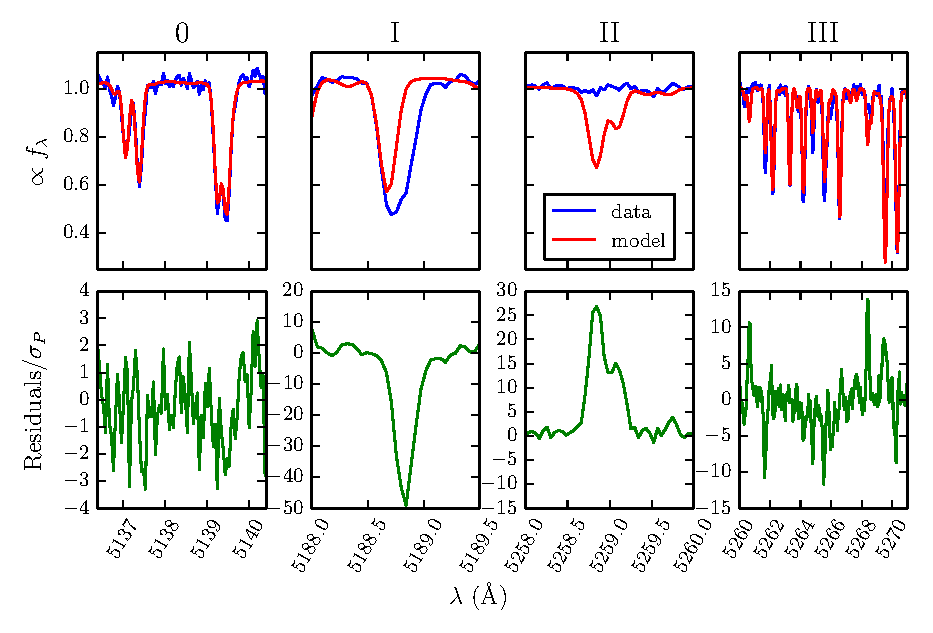
\includegraphics{lineclasses}
\caption{The four classes of line behavior, from left to right: \textbf{Class 0}: the model behaves as expected. \textbf{Class I}: a spectral line is present in the data but missing from the model (in this case, the line is also blended). \textbf{Class II}: a spectral line exists in the model where there is only continuum in the data. \textbf{Class III}: lines exist in both the data and model, however they are of the wrong strength. Some lines are too strong while others are too weak. The lower panels show the residual spectra in units of the observational uncertainty (Poisson uncertainty only).}
\label{fig:lineclasses}
\end{center}
\end{figure}

\subsection{Classes of synthetic spectral line behavior}
From our forward modelling experiments using the modified Kurucz grid used in \citet{blj+12} and the recent PHOENIX grid \citep{hwd+13}, we have identified ways that synthetic spectra diverge from the our observed data. To start, we will describe these classes of behaviour as being tied to specific spectral lines present against a well-defined continuum. Later on, we will use the classes to describe features more generally to cover the behavior of molecular features in later type spectra. See Figure~\ref{fig:lineclasses} for visual examples of each class of behavior.

\paragraph{Class 0} These lines actually produce a good fit with a residual nearly consistent with the Poisson counting uncertainty (see \S\ref{sec:TRES} for how the data is processed). If every region of the spectrum behaved like this, we might be justified in using a $\chi^2$ likelihood function and calling it a day.

\paragraph{Class I} A spectral line appears in the data but not in the model spectrum over a wide range of probable stellar parameters (1000 K in $T_{\rm eff}$, and 1 dex in $\log(g)$, $\Z$, and $\A$. Such a type of error is perhaps the easiest to understand and to forgive. For example, such a line could easily appear in the data due to interstellar absorption or telluric absorption, something which a stellar model could never produce. The model could also fail to reproduce a true stellar line due to a missing opacity source.

\paragraph{Class II} A spectral line appears in the model but not in the data over a wide range of probable stellar parameters (1000 K in $T_{\rm eff}$, and 1 dex in $\log(g)$, $\Z$, and $\A$. This is a more puzzling error, because presumably atomic constants would be much more likely to be \emph{missing} than added in by accident. Presumably this might be a combination of incorrect atomic data coupled with incorrect atmospheric structure that incorrectly excites a line.

The traditional way to account for Class I and Class II errors is to sigma clip the bad lines in the spectrum \citep{kpb+09, mga13}. A region of the spectrum with Class I or II errors is useless for determining spectral parameters. While sigma-clipping routines are to be avoided, if they can correctly mask these regions, then at least they are moving in the right direction.

There is additional information available to help determine which regions of the spectrum suffer from Class I or II errors.For a normal star with absorption lines against a continuum, Class I residuals will always be negative and not change significantly with $\vg$, since we the model can only produce continuum in that region. Class II residuals will always be positive and their magnitude should decrease with decreasing metallicity, since lower metallicity will decrease the strength of all lines. We could easily store the partial derivatives of an individual synthetic spectrum with respect to $\vg$
\begin{equation}
  \bigl \{ \frac{\partial \fM(\lambda | \vg)}{ \partial T_{\rm eff}}, \frac{\partial \fM(\lambda | \vg)}{ \partial \log(g)}, \frac{\partial \fM(\lambda | \vg)}{ \partial \Z}, \frac{\partial \fM(\lambda | \vg)}{ \partial \A} \bigr \}
  \label{eqn:derivative}
\end{equation}
and coupled with a prior on the range of parameters over which the residuals will be correlated, we could shore up the classification of Class I and II errors. 

\paragraph{Class III} errors occur when the line strengths between the data and model do not match at a $\vg$ that fits a majority of the other lines. What makes Class III errors truly pernicious is that for a specific line, there does exist a set of $\vg$ that could properly fit the line, though this parameter combination would result in bad fits for the majority of the other lines. Class I and II errors are easy to identify since the lines will always be bad across a wide range of $\vg$ and have predictable behaviors with change in $\vg$. Class III errors, however, come in both directions: the line can be too strong or too weak. Identifying Class III errors requires making a choice about which lines to trust and how much. 

Most of the Class III errors can probably be identified by finding the regions of the spectrum that have the highest residuals after dealing with Class I and II errors, although some mildly incorrect Class III lines will be difficult to distinguish from correct (Class 0) lines that are simply fit with a less probable $\vg$. Once identified, properly handling Class III errors requires careful thought because these regions of the spectrum \emph{still contain information about $\vg$}. If we take an masking approach as with Class I and II errors, we will be throwing it away. It might even be the case that Class III regions contain \emph{the most} information about $\vg$, since these ``delicate regions'' are the most sensitive to changes in $\vg$ at that particular $\vg$ and thus are tricky to tune correctly. In other words, Class III regions might also be regions where the spectrum derivative (Eqn~\ref{eqn:derivative}) is largest.

To summarize, the fundamental problem with comparing high resolution stellar spectra to grids of synthetic stellar spectra is that no one model $\vg$ will fit all of the lines properly. One can either limit their fits to regions of the spectrum that they know their spectral libraries to be accurate (implicitly masking the rest and potentially discarding a large amount of information) or suck it up and forward model the regions where the models perform poorly.


\section{Instrumental effects and ``nuisance'' parameters in the limit of a perfect stellar model}
\label{sec:perfect}
While this document aims to be general in scope, any forward-modelling approach must also discuss the characteristics of the instrument that performed the observations. We are currently modelling data obtained with the \emph{TRES}\footnote{\url{http://tdc-www.harvard.edu/instruments/tres/}} echelle spectrograph, and so we will describe the characteristics of the instrument and the calibration approaches we have taken, although we note that our approach is easily generalized for data obtained with other spectrographs.

\emph{TRES} is a 51-order echelle spectrograph on the 1.5-m Tillinghast reflector at Whipple Observatory. It spans the full optical range ($3800-9000$\AA) at a resolution of $R=48,000$ ($6.8\;{\rm km/s}$). Echelle spectrographs impart a strong blaze function upon each order, where transmission is largest in the center of the order and declines rapidly as one moves towards the edge of the order. The \emph{TRES} pipeline extracts orders such that they span a wavelength region until the transmission reaches $\lesssim$ 25\% of the central transmission in that order. Each order spans $\sim 100$\AA\ and the blue orders overlap while there are gaps between the wavelength coverage of the red orders. This spectra are blaze-corrected by dividing by a blaze function determined from fitting nightly exposures of flat lamps. Then, the spectrum is flux calibrated using sensitivity functions determined from nightly observations of spectrophotometric standards (O stars). The flux-calibrated spectrum is in units of ergs/s/${\rm cm}^2$/\AA.

\paragraph{Processing TRES Data}
\label{sec:TRES}
Because the \emph{TRES} reduction pipeline does not produce a ``sigma spectrum'' like that determined by a standard IRAF reduction, we instead calculate the Poisson uncertainty on each pixel. We can find the signal-to-noise ratio of each pixel using the raw (still-blazed) spectrum, which is in units of ``counts.''
\begin{equation}
  [S/N](\lambda) = \sqrt{ {\rm cts}(\lambda)}
\end{equation}
the Noise-to-Signal ratio is the inverse 
\begin{equation}
  [N/S](\lambda) = \frac{1}{\sqrt{ {\rm cts}(\lambda)}}
\end{equation}
To determine the uncertainty of the flux-calibrated spectrum, we multiply by N/S. The $[N/S](\lambda)$ ``spectrum'' is larger at the edges of each order due to the reduced transmission. Please note that statistic pixel uncertainties derived in this manner neglect regions of the spectrum that might have a higher variance due to sitting atop a night sky line, but short of implementing our own reduction pipeline for \emph{TRES}, there isn't much more we can do at the moment.

\paragraph{Generating a model spectrum} We parameterize the fit to a star by $\vt = \{\vstar, \vN \}$, where stellar parameters include $\vstar = \{T_{\rm eff}, \log(g), \Z, \A, v \sin i, v_z, A_v, R_\star^2/d^2 \}$. The data vector $\vD = \fD(\lambda)$ represents the \emph{TRES} spectrum. To generate a model spectrum given a set of parameters $\fM(\vt)$, a model spectrum is created by first linearly interpolating in $T_{\rm eff}, \log(g), \Z, \A$ space between grid points of instrumentally broadened and oversampled synthetic stellar spectra. Then, the spectrum is rotationally broadened for $v \sin i$ using Fourier techniques, Doppler shifted by $v_z$, extinction corrected for $A_V$, multiplied by $R_\star^2/d^2$ for a solid angle correction, and finally downsampled to the exact pixels of the TRES spectrum using spline interpolation\footnote{Because we are dealing with flux-calibrated data and synthetic spectra, we \emph{resample} to lower resolution. We do not \emph{rebin} because we are dealing with flux-density, not photon counts}.

FIGURE: showing the high resolution, raw $R =$ 500,000 spectrum compared to the one convolved with a kernel down to $R =$ 50,000. This shows that lines are blended, but it is important to keep in mind that we do have access to the high resolution models when talking about bad pixels or bad line-species. For example, we could inject bad lines in this high resolution space.

\subsection{Applied to a Gaussian likelihood function}
For the rest of \S\ref{sec:perfect}, we proceed as if there were no Class I, II, or III errors present in our model so that we may illustrate our technique for dealing with uncertainties in the flux-calibration. Although per-pixel photon counting errors are Poisson, we can safely assume that we have enough counts that we are in the Gaussian limit, although see the discussion in \S\ref{sec:residuals}. Then our likelihood function becomes a pixel-by-pixel $\chi^2$ comparison between the data spectrum $\fD$, and the model spectrum $\fM$, summed over the wavelength axis. 
\begin{equation}
 p(\vD | \vt) = {\cal L} \propto \exp \left(-\frac{\chi^2}{2} \right)
\end{equation}
\begin{equation}
  \chi^2 = \sum_\lambda \left [\frac{ \fD(\lambda) - k(\lambda | \vN) \fM(\lambda | \vstar) }{\sigma(\lambda)} \right ]^2
\end{equation}
With flat priors on $\vstar$ and $\vN$ (an assumption we will later relax) the logarithm of our posterior probability function is then
\begin{equation}
  \ln \bigl [p(\vt | \vD) \bigr] \propto - \frac{1}{2} \sum_\lambda \left [\frac{ \fD(\lambda) - k(\lambda | \vN) \fM(\lambda | \vstar) }{\sigma(\lambda)} \right ]^2
  \label{eqn:lnprob}
\end{equation}

The prefactor $k(\lambda | \vN)$ is a calibration function that aims to account for errors in the blaze-correction or flux-calibration by multiplying the synthetic spectrum by a polynomial. The parameters describing this function are the coefficients of the polynomial. This approach of accounting for large-scale calibration errors in the spectrum is more justified than the traditional approach of normalizing to the stellar continuum. From a flux-calibration experiment where we observed spectrophotometric standards BD+28 and BD+25 multiple times, we calibrated the dispersion in (FIGURE showing the sensitivity function for a few representative orders) flux-calibration function, or IRAF's ``sensitivity function.'' These tests revealed that the largest source of error in flux-calibration was actually in the overall magnitude of individual order, this could be due to slit losses, poor correction due to parallactic angle, or scattered light within the instrument. These corrections are smaller than 10\%. But more importantly, the corrections in the higher order terms (ie, the shape of the bandpass calibration for each order) are small ($\lesssim 3\%$). As described in \S\ref{sec:priors}, we can set priors on these coefficients. This prior information on the calibration parameters motivates our choice of functional parameterization for the nuisance parameters in \S\ref{sec:nuisance}.
The polynomial approach is also better than the normalization approach if the order only spans a small region of the spectrum. If a M star absorption band spanned the whole order, one might accidentally normalize to the feature rather than a pseudo-continuum.


\subsection{Nuisance parameters}
\label{sec:nuisance}
In our case, $\vN = \{c_0, c_1, \ldots, c_N\}$ are a set of 4 Chebyshev polynomial coefficients for each order. This amounts to a ``re-fluxing'' of the model following the techniques of \citet{elh+06}. We apply the re-fluxing to the model rather than attempt to re-flux the data since this operation would also need to re-scale the noise, making $\chi^2$ a complicated function of $k$.


In order to understand the effects of the $k(\lambda | \vN)$ term, we now consider its effects on just one order of the 51-order echelle spectrum. The first four Chebyshev polynomials are 
\begin{align*}
  T_0(x) &= 1\\
  T_1(x) &= x\\
  T_2(x) &= 2 x^2 - 1\\
  T_3(x) &= 4 x^3 - 3x\\
\end{align*}
In our implementation, we map the full pixel range of a specific order $\lambda \in [\lambda_{\rm min}, \lambda_{\rm max}]$ to $x \in [-1, 1]$. By mapping pixel number in a given order, rather than wavelength, we are insensitive to wavelength shifts of the model. Then, for a given set of Chebyshev coefficients, $\vN = \{ c_0, c_1, c_2, \ldots, c_N \}$, we have 
\begin{align}
  k(\lambda | \vN) &= c_0 T_0(\lambda) \left [1 + c_1 T_1(\lambda) + \ldots + c_N T_N(\lambda) \right ]\\
  k(\lambda | \vN) &= c_0 \left [1 + \sum^N_{i = 1} c_i T_i(\lambda) \right ]
  \label{eqn:k_new}
\end{align}
When applied to scale the model flux $\fM$, this becomes
\begin{align}
  k(\lambda | \vN) \fM &=  \left [1 + \sum^N_{i = 1} c_i T_i(\lambda) \right ] (c_0 \fM)\\
  k(\lambda | \vN) \fM &= c_0 \fM + c_1 T_1 (c_0 \fM) + \ldots + c_N T_N (c_0 \fM)
\end{align}

This functional form of $k$ allows $c_0$ to scale by large amounts while the higher order terms (denoted by $c_n$) are perturbations on top of the \emph{scaled} model ($c_0 \fM$). However, see \S\ref{sec:gaussian_simplification} for an alternative model when perturbations are small. We can rewrite Equation~\ref{eqn:lnprob} as 
\begin{equation}
  \ln \bigl [p(\vt | \vD) \bigr] \propto - \frac{1}{2} \sum_\lambda \left [\frac{\fD(\lambda) - \bigl [1 + \sum^N_{i = 1} c_i T_i(\lambda) \bigr ] c_0 \fM(\lambda | \vstar)  }{\sigma(\lambda)} \right ]^2
  \label{eqn:lnprob2}
\end{equation}
To simplify the following discussion, we consider a single wavelength $\lambda_i$ and then generalize this to a sum over $\lambda$ later. If we expand out the square in Equation~\ref{eqn:lnprob2}, then for a given $\lambda_i$ we have
\begin{equation}
  \ln \bigl [p(\vt | \lambda_i) \bigr] \propto -\frac{1}{2 \sigma^2} \left [ \fD^2 - 2 \fD c_0 \fM \left [1+ \sum_{i=1}^N c_i T_i \right ]+ c_0^2 \fM^2 \left [1 + \sum_{i=1}^N c_i T_i \right ]^2 \right ]
 \label{eqn:lnprob_lambda}
 \end{equation}
where $\sigma$, $\fD$, $\fM$, and $T_{n,m}$ are all evaluated at $\lambda_i$. We can further expand this to
\begin{equation}
  \ln \bigl [p(\vt | \lambda_i) \bigr] \propto - \frac{1}{2 \sigma^2} \left [ \fD^2 - 2 \fD c_0 \fM \left [1+ \sum_{i=1}^N c_i T_i \right ]+ c_0^2 \fM^2 \left [1 + 2 \sum_{i=1}^N c_i T_i + \sum_{i=1}^N \sum_{j=1}^N c_i T_i c_j T_j \right ] \right ]
  \label{eqn:expanded}
 \end{equation}

To simplify this math, we can rewrite the Chebyshev coefficients and polynomials as column vectors $\vc$ and $\vec{T}(\lambda)$, respectively
\begin{equation}
  \vc = 
  \begin{bmatrix}
    c_1\\
    c_2\\
    \vdots\\
    c_N
  \end{bmatrix}
  \hspace{3cm}
\vec{T}(\lambda) = 
\begin{bmatrix}
T_1(\lambda)\\
T_2(\lambda)\\
\vdots\\
T_N(\lambda)\\
\end{bmatrix}
\end{equation}
then 
\begin{equation}
  k(\lambda | \vN) = c_0 \left [ 1 + \sum^N_{i = 0} c_i T_i \right ] = c_0 \left[ 1+ \vec{T}^\trans \cdot \vc \right]
\end{equation}
If we let 
\begin{equation}
  {\bm W}(\lambda) = \vec{T} \cdot \vec{T}^\trans = 
  \begin{bmatrix}
T_1 T_1 & T_1 T_2 &  \hdots & T_1 T_N \\
T_2 T_1 & T_2 T_2 &  \hdots & T_2 T_N \\
\vdots  & \vdots  &  \ddots & \vdots \\
T_N T_1 & T_N T_2 &  \hdots & T_N T_N \\
  \end{bmatrix}
\end{equation}
then we have
\begin{equation}
  \sum_{i =1}^N \sum_{j=1}^N c_i T_i c_j T_j = \vc^\trans \cdot {\bm W} \cdot \vc
\end{equation}
We can rewrite Equation~\ref{eqn:expanded} quthat should be accounted for? adratically in $\vc$ as
\begin{equation}
  \ln \bigl [p(\vt | \lambda_i) \bigr] \propto - \frac{1}{2 \sigma^2} \left [ \fD^2 - 2 \fD c_0 \fM \left [1+ \sum_{i=1}^N c_i T_i \right ]+ c_0^2 \fM^2 \left [1 + 2 \sum_{i=1}^N c_i T_i + \sum_{i=1}^N \sum_{j=1}^N c_i T_i c_j T_j \right ] \right ]
 \end{equation}
\begin{equation}
  \ln \bigl [p(\vt | \lambda_i) \bigr] \propto - \frac{1}{2} \frac{c_0^2 \fM^2}{\sigma^2} \sum_{i=1}^N \sum_{j=1}^N c_i T_i c_j T_j + \left (\frac{- c_0^2 \fM^2 + c_0 \fD \fM}{\sigma^2} \right ) \sum_{i=1}^N c_i T_i  -  \left( \frac{c_0^2 \fM^2 - 2 c_0 \fD \fM + \fD^2}{2 \sigma^2} \right)
\end{equation}
\begin{equation}
  \ln \bigl [p(\vt | \lambda_i) \bigr] \propto - \frac{1}{2} \frac{c_0^2 \fM^2}{\sigma^2}  \vc^\trans {\bm W} \vc + \left (\frac{- c_0^2 \fM^2 + c_0 \fD \fM}{\sigma^2} \right ) \vec{T}^\trans \vc -  \left( \frac{c_0^2 \fM^2 - 2 c_0 \fD \fM + \fD^2}{2 \sigma^2} \right)
\end{equation}

Because matrix multiplication is associative, we can sum ${\bm W(\lambda)}$ and $\vec{T}^\trans(\lambda)$ across all $\lambda$, and define
\begin{align}
  {\bm A} &= c_0^2 \sum_{\lambda} \frac{\fM^2(\lambda)}{\sigma^2(\lambda)} {\bm W}(\lambda) \\
  \vec{B} &= \sum_{\lambda} \frac{-\fM^2(\lambda) c_0^2 + \fD(\lambda) \fM (\lambda) c_0}{\sigma^2(\lambda)} \vec{T}(\lambda)\\
  g &= -\frac{1}{2} \sum_{\lambda} \frac{c_0^2 \fM^2(\lambda) - 2 c_0 \fD(\lambda) \fM(\lambda) + \fD^2(\lambda)}{\sigma^2(\lambda)} 
\end{align}
Where ${\bm A}$, $\vec{B}$, and $g$ are each a function of $\vstar$, $\vN$, and $\vD$. Now we can rewrite Equation~\ref{eqn:lnprob2} as 
\begin{align}
  \ln \bigl [p(\vstar, \vN | \vD) \bigr] &\propto - \frac{1}{2} \vc^\trans {\bm A} \vc + \vec{B}^\trans \vc + g\\
  p(\vt | \vD) = p(\vstar, \vN | \vD) &\propto \exp \left ( - \frac{1}{2} \vc^\trans {\bm A} \vc + \vec{B}^\trans \vc + g \right )
  \label{eqn:lnprob_matrix}
\end{align}
Here we have the full posterior probability distribution assuming flat priors. This posterior is a function of both the stellar parameters $\vstar$ and the nuisance parameters $\vN$. Generally, we are most interested in the stellar parameters after they have been marginalized over the nuisance parameters. This marginalization encapsulates the uncertainty due to the inference on the nuisance parameters. Because this probability function is a multi-dimensional Gaussian in the higher order Chebyshev coefficients $\vc = \{c_1, c_2, \ldots, c_N \}$, we can do this marginalization analytically, and then sample from the marginalized distribution. 
\begin{equation}
  p(\vstar, c_0 | \vD) = \int p(\vstar, c_0, \vc\; | \vD) \dd \vc
\end{equation}
The analytic multi-dimensional Gaussian integral with linear term \citep{sgd+09} yields 
\begin{align}
  p(\vstar, c_0 | \vD) &\propto \int \exp \left ( - \frac{1}{2} \vc^\trans {\bm A} \vc + \vec{B}^\trans \vc + g \right ) \dd \vc\\
  p(\vstar, c_0 | \vD) &\propto \sqrt{\frac{(2 \pi )^N}{ {\rm det} \bigl |{\bm A} \bigr |}} \exp{ \left ( \frac{1}{2} \vec{B}^\trans {\bm A}^{-1} \vec{B} + g \right )}
\end{align}
Where $N$ is the number of Chebyshev coefficients marginalized over, in our case $N=3$. By doing this marginalization we have reduced the dimensionality of our posterior space from $200+$ parameters ($\sim 7$ stellar parameters plus 3 Chebyshev coefficients for each of 51 echelle orders) to $\sim 60$ ($\sim 7$ stellar parameters and one $c_0$ for each of the 51 echelle orders). This enables a dramatic speedup in the MCMC sampling. For flux-calibrated spectra where the variation in $c_0$ is expected to be small (less than how much?), we can approximate $k$ in a different manner which allows marginalization over the $c_0$ coefficients as well, reducing the dimensionality of the space to only the $\sim 7$ stellar parameters. This approach is detailed in \S\ref{sec:gaussian_simplification}.


\subsection{Including Gaussian priors on nuisance parameters}
\label{sec:priors}
Using this polynomial formalism, it is possible to incorporate prior knowledge about the degree of necessary ``re-fluxing'' through priors on the nuisance parameters. From our flux-calibration experiment, we determined that the overall scaling could range by 10\%, while the higher order corrections were less than 3\%. Because $c_0$ is a scale factor, it should be equally probable to scale up by a factor of two as it is to scale down by a factor of two. This means we should be using a log-normal prior on $c_0$
\begin{align}
  p(c_0) &= \frac{1}{\sqrt{2 \pi} \sigma_{c_0} c_0} \exp \left( -\frac{(\ln c_0)^2}{2 \sigma_{c_0}^2} \right) \\
  \ln p(c_0) &= \ln \left( \frac{1}{\sqrt{2 \pi} \sigma_{c_0} c_0} \right) - \frac{(\ln c_0)^2}{2 \sigma_{c_0}^2}
\end{align}
centered on $c_0 = 1$. Because the higher order polynomial terms are perturbations on the scaled model ($c_0 f$), we assume Gaussian priors centered about 0
\begin{equation}
  p(c_n) = \frac{1}{\sqrt{2 \pi} \sigma_{c_n}} \exp \left( - \frac{c_n^2}{2 \sigma_{c_n^2}} \right)
\end{equation}
which we can express in vector form as
\begin{equation}
  p(\vc\;) \propto \exp \left ( -\frac{1}{2} (\vc - \vec{\mu})^\trans {\bm D} (\vc - \vec{\mu}) \right )
  \label{eqn:nuisance_prior} 
\end{equation}
where 
\begin{equation}
  {\bm D} = 
  \begin{bmatrix}
    \sigma_1^{-2} & 0 & \hdots & 0 \\
    0 & \sigma_2^{-2} & \hdots & 0 \\
    \vdots & \vdots & \ddots & 0 \\
    0 & 0 & \hdots & \sigma_N^{-2} \\
  \end{bmatrix}
\end{equation}
and $\sigma_i$ represents the width of the Gaussian prior on the i-th Chebyshev coefficient, in our case $\sigma_i = \sigma_{c_n} \approx 0.03$. $\vec{\mu}$ is the mean of the Gaussian prior, in nearly all cases we expect to set this to $\vec{\mu} = \{0, 0, \ldots, 0\}$, unless we have prior knowledge that the flux-calibration is systematically warped in one direction. Now, we can write the posterior with priors as
\begin{equation}
  p(\vstar, \vN | \vD) = p(\vstar, c_0, \vc\; | \vD) \propto p( \vD | \vstar, c_0, \vc\; ) p(\vc\;) p(\vstar) p(c_0) 
\end{equation}
\begin{equation}
  p(\vstar, \vN | \vD) \propto \exp \left ( - \frac{1}{2} \vc^\trans {\bm A} \vc + \vec{B}^\trans(\vstar) \vc + g(\vstar) \right )  \exp \left ( -\frac{1}{2} (\vc - \vec{\mu})^\trans {\bm D} (\vc - \vec{\mu}) \right ) p(\vstar) p(c_0)
  \label{eqn:posterior_prior}
\end{equation}
we can expand and rearrange the argument of Equation~\ref{eqn:nuisance_prior} to a similar form that is quadratic in $\vc$
\begin{align}
  -\frac{1}{2} (\vc - \vec{\mu})^\trans {\bm D} (\vc - \vec{\mu}) &= \frac{1}{2}\left ( -\vc^\trans {\bm D} \vc + \vc^\trans {\bm D} \vec{\mu} + \vec{\mu}^\trans {\bm D} \vc - \vec{\mu}^\trans {\bm D} \vec{\mu} \right )\\
  &= -\frac{1}{2} \vc^\trans {\bm D} \vc + ({\bm D} \vec{\mu})^\trans \vc - \frac{1}{2} \vec{\mu}^\trans {\bm D} \vec{\mu}
\end{align}
then we can rewrite
\begin{align}
  {\bm A}^\prime &= {\bm A} + {\bm D}\\
  \vec{B}^\prime &= \vec{B} + ({\bm D} \vec{\mu})^\trans\\
  g^\prime &= g - \frac{1}{2} \vec{\mu}^\trans {\bm D} \vec{\mu} 
\end{align}
in the case that $\vec{\mu} = \{0, 0, \ldots, 0\}$, there is only a non-zero correction to ${\bm A}$. The full posterior probability distribution is then
 \begin{equation}
   \boxed{
  p(\vstar, \vN | \vD) = p(\vstar, c_0, \vc\;) \propto \exp \left ( - \frac{1}{2} \vc^\trans {\bm A}^\prime \vc + \vec{B}^{\prime \trans} \vc + g^\prime \right ) p(\vstar) p(c_0) p(\vc)
}
\label{eqn:lnprob_lognormal}
\end{equation}
This probability function appears in the code as \texttt{lnprob\_lognormal} and has $\sim 7$ stellar dimensions and $\sim 200$ nuisance dimensions.

Using the previous multi-dimensional integral, we can marginalize over the $\vc$ including the Gaussian priors
\begin{equation}
  \boxed{
  p(\vstar, c_0 | \vD) \propto \sqrt{\frac{(2 \pi )^N}{ {\rm det} \bigl |{\bm A}^\prime \bigr |}} \exp{ \left ( \frac{1}{2} \vec{B}^{\prime\trans} {\bm A}^{\prime -1} \vec{B}^\prime + g^\prime \right )} p(\vstar) p(c_0)
}
\label{eqn:lnprob_lognormal_marg}
\end{equation}
where $N$ is the number of Chebyshev coefficients marginalized over, in our case $N=3$. This probability function appears in the code as \texttt{lnprob\_lognormal\_marg} and has $\sim 7$ stellar dimensions and $\sim 50$ nuisance dimensions. If we increase the permissible degree of re-fluxing by increasing $\sigma_i$, this will have the effect of smearing out or widening the posterior on a given $\vstar$.

If one uses a marginalized posterior, but is still interested in obtaining a flux-corrected spectrum for the purposes of inspecting the residuals, it is still possible to do so. We can use Eqn~\ref{eqn:lnprob_lognormal} with $\vstar$ fixed at a sample from the posterior of Eqn~\ref{eqn:lnprob_lognormal_marg} and then use MCMC to draw samples from $p(\vN | \vstar, \vD)$. Now, the combination of $\vstar$ and $\vN$ completely describes a flux-corrected spectrum.

\subsection{Sampling a un-flux calibrated model}
There also exists a wealth of archival \emph{TRES} data that is not flux calibrated, since its primary purpose was for radial velocity determination of FGK stars. To fit this data we can use newer sensitivity functions taken under different conditions and soften the priors on the coefficients. Tests indicate that this works rather well. The blaze function will might change significantly between nights and years, so this might be a source of error.

For non flux calibrated spectra, we determined that the overall spread in $c_0$ across all orders should not be more than $\sigma_{c_0} \leq 2$, or the one-sigma deviation of $c_0$ is between $0.125 \leq c_0 \leq 8.0$. The plot in plots/priortests shows that log-normal prior (vs. Gaussian) on $c_0$ is the correct choice . Since we care most about the inference on F, we want to know that this prior is not biasing the final outcome. Using a Gaussian prior with a large $\sigma_{c_0}$ will bias the results, but if $\sigma_{c_0}$ is small ($\lesssim 0.2$), then we can get away with Gaussian priors (see \S\ref{sec:gaussian_simplification}). Is there a better way to determine these thresholds other than my current technique of testing and visual inspection?
 
\subsection{Hierarchical modelling}
Instead of the current framework where the nuisance coefficients of each order are independent, we could derive a hierarchical framework where each $c_0$ is drawn from a probability distribution of $c_0$ described by a hyperparameter $C_0$. If each order required a similar $c_0$, then this would enable shrinkage of $C_0$, however if each order required a widely disparate $c_0$, then $C_0$ would correspondingly increase. Higher order coefficients could still be analytically marginalized over. 

\subsection{Sampling the posterior and performance of the $\chi^2$ likelihood}
Currently we are sampling this posterior with the MCMC ensemble sampler \citep{gw10} implemented in \texttt{Python} by \citet{fhl+12} as \texttt{emcee}. See \citet[CosmoHAMMER]{asa+13} for a review of \texttt{emcee} parallel performance and scaling relationships on a computer cluster. 

In this section, we described our approach to take into account flux calibration errors assuming a perfect synthetic spectra. If one does a straight up $\chi^2$ fit to the data, however, you can get posteriors that look have 1-sigma contours of $\pm 1$ K and $\pm 0.01$ dex in gravity and metallicity. This would be as precise as stellar parameters obtained with astroseismology! Clearly there is something going wrong here.

As our previous discussion has noted, these posteriors are unfortunately too good to be true and we must take a more sophisticated approach. However, many of the flux-calibration principles developed in this section should still apply. More advanced posterior functions in the following sections might require using more specialized MCMC techniques such as Gibbs sampling or expectation maximization (EM). 

\section{Baby steps beyond a perfect stellar model}
\label{sec:residuals}
In this section we describe a few simple things we might try (or have tried) in order to remedy the shortcomings of the previous section.

\subsection{Additional sources of noise}
Presumably we shouldn't have to add an additional source of instrumental ``noise'' to the fit, because our nuisance parameters will find an exact flux calibration. However, CCD readnoise and 1D spectrum extraction will almost definitely increase the noise in a pixel beyond theoretical Poisson limits. Normally this information will be encapsulated in a ``sigma spectrum,'' but unfortunately we do not have access to this unless we develop an alternative to the \emph{TRES} pipeline. We could try to fudge adjustments to the readout noise by adding a small error in quadrature.

Even the stellar continuum can flicker/jitter (as shown by Kepler studies), which would produce a small departure from a perfect continuum. Even in the Class 0 region of our spectrum (Figure~\ref{fig:lineclasses}, left panel), the residuals are slightly larger than 1 $\sigma$ on average.

When we interpolate a synthetic spectrum from the library to a specific $\vg$, we will introduce interpolation errors depending on how close we are to a grid point in the library. \citet{hus12} investigate the possible range of interpolation errors at specific $\vg$ by dropping out a spectrum from the grid, interpolating over it, and then comparing the true spectrum to the interpolated spectra. For hotter stars with well defined continua, we find the maximum error is $\lesssim 5$\%, while for M stars the error could be as large as $\sim 20$\% for some spectral features. By doing this interpolation test across the grid, we could determine an ``interpolation error spectrum'' that would encapsulate the maximum error possible for an interpolated spectrum, weighted by its distance from the nearest grid points. This uncertainty could be included in quadrature. Since most of our \emph{TRES} spectra are at signal/noise of $\sim 30$ per pixel (or noise/signal ratio of $1/30 \approx 0.03$), an interpolation noise contribution of $\sim 5$\% the level of the signal level would be significant. However, we tried arbitrarily increasing the Poisson errors by a factor of 2 or 3 and it didn't significantly change the results. While such an error spectrum should eventually be incorporated, we have bigger fish to fry. 

\subsection{Masking}
We must necessarily mask certain wavelength regions of the T Tauri spectra that are contaminated (one might also say ``made more interesting'') by the astrophysical realities of accretion or stellar spots (such as the Balmer lines, which are in emission).  We also accept the assumption that rotation or accretion onto the star does not fundamentally alter the structure of the model atmosphere that generates the model spectrum and that a spectral comparison of the ``clean'' regions of the spectrum is valid. We also mask blatant Class I and II regions by eye, but currently do nothing for smaller errors or Class III errors.

\subsection{Gallery of likelihood functions}
A problem with the $\chi^2$ likelihood function is that the Gaussian tails of the probability function rapidly decline, making any outliers extremely improbable, which will bias a fit. 

A common approach to make ``robust inference'' is to use a likelihood function with fatter tails. Although not rigorously motivated, this is can be a quick thing to try. We explore the following likelihood functions.

\paragraph{Combination of Gaussian with exponential wings}
We fit a function of the form
\begin{equation}
  p(\fD(\lambda) | \fM(\lambda | \vt)) \propto \exp \left (\frac{(\fD - \fM)^2}{(\sigma_G \sigma_P)^2} \right ) + A \exp \left (\frac{|\fD - \fM|}{\sigma_E \sigma_P}  \right )
\end{equation}
to the residuals of a reasonable $\vt$ to determine $A$, $\sigma_G$, and $\sigma_E$. This functional form assumes that there will be a Gaussian core, similar to the $\chi^2$ likelihood, but also allows some contribution from an exponential tail, used to describe the residuals. I think the problem here is that the exponential is too steep to properly describe Class I and II residuals, although it might do well for Class III errors.

\paragraph{Sivia's model}
\citet{ss06} describe a likelihood function which treats the noise estimate for each data point suspiciously. The true noise $\sigma$ can be no smaller than some original estimate $\sigma_0$, but it may be much larger. By putting a prior on $\sigma$, 
\begin{equation}
  p(\sigma | \sigma_0) = \left \{ \begin{array}{cc}
    \sigma_0/\sigma^2 & \sigma  \leq \sigma_0\\
    0                 & \textrm{else}
  \end{array}
    \right.
\end{equation}
and marginalizing over the $\chi^2$ likelihood, the new likelihood function becomes
\begin{equation}
  p(\fD | \fM, \sigma_0) = \frac{1}{\sigma_0 \sqrt{2 \pi}} \left [ \frac{1 - e^{-R^2/2}}{R^2} \right ] 
\end{equation}
where $R = (\fD - \fM)/\sigma_0$. This function has even fatter tails than the exponential model and seems to give more believable results. We have done the most testing using this new likelihood function, but it still does not give a truly satisfying result. For example, which lines contributed most to the posterior? What about the wings of class I and II errors? These individual pixels might still be given a weight of $\sigma_0$ because they are not nearly as bad as the line centers.

\paragraph{$\chi^2$ with flat tails}
\citet{hbl10} describe a likelihood function that smoothly caps the total likelihood contribution any outlier might have at some constant $Q$ by using a $\chi^2_Q$ function
\begin{equation}
  \chi^2_Q = \sum_{i = 1}^N \frac{Q^2 [\fD - \fM]^2}{Q^2 \sigma_P^2 + [\fD - \fM]^2}
\end{equation}
In some ways, this is analogous to sigma-clipping. Once a residual reaches the flat tails, it fails to factor into the determination of parameters.

Other functions we might try include a Student-t statistic, a Lorentzian, or a linear combination of Gaussians. While all of these likelihood function shenanigans are amusing, we would like to move beyond tweaking the fitting function towards an approach that properly incorporates knowledge about the specifics of our problem.

\subsection{Bad data model}
The bad data model \citep{pre97,hbl10} is a powerful framework for forward modelling data, which allows the modeler to explicitly account for outliers using a generative model.

In the simplest mixture model, each data point has a binary flag $q_i$ which specifies whether that data point is good or bad. Then, for the entire data set we have an ensemble of $\qN$. If this ensemble of $\qN$ is chosen appropriately, and the good data points are flagged as good and the bad data points are flagged as bad, the likelihood will be maximized. We adopt $P_B$ for the \emph{a priori} probability that a given data point will be bad, $Y_b$ for the mean of the bad data distribution, and $V_b$ for its variance. Written out explicitly, this is
\begin{multline}
  {\cal L} = p({\bm D} | \vt,\qN, Y_b,V_b) = \prod_{i=1}^N \left [ \frac{1}{\sqrt{2 \pi} \sigma} \exp \left[ - \frac{(\fD - \fM)^2}{2 \sigma^2} \right] \right ]^{q_i}  \times \\
  \left [ \frac{1}{\sqrt{2 \pi (V_b + \sigma^2)}} \exp \left[ - \frac{(\fD - Y_b)^2}{2 (V_b + \sigma^2)} \right]
  \right ]^{1 - q_i}
\end{multline}
We we a Bernoulli prior on the $q_i$
\begin{equation}
  p(q_i | P_b) = [1-P_b]^{q_i} P_b^{[1-q_i]}
\end{equation}
then, the probability of any given ensemble of $\qN$ is 
\begin{equation}
  p(\qN | P_b) = \prod_{i=1}^N [1-P_b]^{q_i} P_b^{[1-q_i]}
\end{equation}

We can analytically marginalize over the single flag by a discrete sum over the two states of $q_i$: $q_i = 1$ and $q_i = 0$. 
\begin{multline}
  p(\vt, P_b, Y_b, V_b | D_i)  =  \int p( \vt, q_i, P_b, Y_b, V_b| D_i) {\rm d} q_i \\
  = p(\vt, q_i=1, P_b, Y_b, V_b | D_i) + p(\vt, q_i=0, P_b, Y_b, V_b | D_i) \\
  = \Bigl[ p_{\rm good}(D_i | \vt)\, p(q_i=1 | P_b) +  p_{\rm bad}(D_i | Y_b, V_b)\, p(q_i=0 | P_b)\Bigr] \times p(\vt ,P_b, Y_b,V_b) 
\end{multline}

\begin{multline}
  p(\vt,P_b,Y_b,V_b|\,{\bm D}) \propto \prod_{i=1}^N \Bigl [ [1 - P_b] p_{\rm good}(D_i |\vt)  + P_b p_{\rm bad}(D_i | Y_b, V_b)\Bigr ] \times p(\vt,P_b, Y_b, V_b)\\
  \boxed{
    = \prod_{i=1}^N \left\{ \frac{1 - P_b}{\sqrt{2 \pi \sigma_{yi}^2}} \exp \left[ - \frac{(\fD - \fM)^2}{2 \sigma^2} \right] + \frac{P_b}{\sqrt{2 \pi (V_b + \sigma^2)}} \exp \left[- \frac{(\fD - Y_b)^2}{2 (V_b + \sigma^2)} \right] \right\}
  \times p(\vt,P_b,Y_b,V_b)}
\end{multline}

In its simplest form, the bad data model results in a likelihood function that is a linear combination of Gaussians. Although the functional form you end up with is similar, the benefit of this bad data approach over a gallery of likelihood functions is that it is motivated by the characteristics of the bad data ($P_B$, $Y_b$, and $V_b$). If we wish to add additional information about the characteristics of the bad data, we can do so. 

\subsection{Spatial correlations of pixels}
We can do more. We now discuss bad data models that leverage more of the information about our problem to more robustly handle systematic errors. In bad model of the previous section, we assumed that each data point is independent. However, we know that Class I, II, and III errors will be correlated across several pixels, where the correlation length is the typical width of a spectral line, set by the stellar rotation kernel $v \sin i$, the instrumental resolution kernel, or both. Some very strong lines (such as the Balmer lines, or the Mg b triplet) will have wings that are correlated across a wider length of pixels.

\subsubsection{Mixture of multiple components}
When we believe that a sample population might be composed of several populations with different behaviours (Class 0, I, II, and III), it makes sense to expand the bad data model to a multiple mixture model. Following \citet{gcs+04}, our likelihood function becomes
\begin{equation}
  p(\fD, \vec{Q} | \vt) = p(\fD | \vec{Q}, \theta) p(\vec{Q}) = \prod_\lambda \prod_{m = 0}^3  {\cal L}_m(\fD(\lambda | \theta_m))^{q_{im}}
\end{equation}
where we use $\vec{Q} = \qM$ to describe a single vector of all the individual $q_{im}$ flags. For example, when a Class I, II, or III error occurs, the core of the line may be a 20 sigma residual while the wings of the line will taper off to a 3 sigma residual, and eventually to a 0 residual once it reaches the continuum. If we treat pixels as uncorrelated, then the small-residual wings of the bad lines might actually have more probability if they were labelled as ``good'' pixels. To remedy this situation, we attempt to develop a bad data model which includes spatial (wavelength) correlations.

This correlation length will probably depend on the spectral type of star. For example, if they're simple F and G stars then the bad lines will likely be singular. But if they are M stars, then there is a chance that there might be a large ``pseudo-continuum'' region that would be incorrect. For Class I and II errors, we could include a hyper parameter describing the width of each line, and another hyper parameter describing the (distribution of) depth. For Class III errors, describing how line strengths might be wrong makes sense for stars with continuum, but as we move to later type stars (K stars) that do not have a nice continuum, we may run into trouble. For the later stars (M dwarfs), there might be a whole region that is incorrect.

Proper Class III modeling is very important, following the discussion of \citep{mga13}. Some spectral features will not fit perfectly, especially at the lower end of the temperature scale. However, it's important to still take these features into account when modelling since they still contain information. How should we account for the fact that some parts of the spectrum carry more information about $\vg$ than other parts of the spectrum? Is it important to weight this parts beforehand? Or should this contribution to the posterior naturally weight itself, the way certain points might heavily contribute to the slope and intercept of a linear fit?

\subsubsection{Correlation of the $q_i$ flags}

In the manner of Gaussian random processes, we develop a covariance function
\begin{equation}
  {\rm cov}(q_i, q_j) = \rho(| \lambda_i - \lambda_j|)
\end{equation}
or where the covariance matrix has components
\begin{equation}
  \Sigma_{ij} = \sigma^2 \rho(|\lambda_i - \lambda_j|)
\end{equation}
where
\begin{equation}
  \rho_{ij} = \frac{ {\rm cov}(i,j)}{\sigma_i \sigma_j} = \frac{E[(X - \mu_x)(Y - \mu_y)]}{\sigma_x \sigma_y}
\end{equation}
that describes the correlation between the state of the bad data flags. The simplest thing to do would be to take the common correlation length in the spectrum imposed by $l$. If we say that the typical feature will have five adjacent pixels wrong, then the correlation matrix would be
\begin{equation}
  \begin{bmatrix}
    1 & 4/5 & 3/5 & 2/5 & 1/5 \\
    4/5 & 1 & 4/5 & 3/5 & 2/5 \\
    3/5 & 4/5 & 1 & 4/5 & 3/5 \\
    2/5 & 3/5 & 4/5 & 1 & 4/5 \\
    1/5 & 2/5 & 3/5 & 4/5 & 1\\
  \end{bmatrix}
\end{equation}
(this is embedded in an N-pixel sparse matrix where everywhere but the diagonal is 0). And so
\begin{equation}
  {\rm cov}(q_i, q_j) = \left \{ \begin{array}{cc}
    1 - \frac{|\lambda_i - \lambda_j|}{5} & |\lambda_i - \lambda_j| \leq 5 \\
    0                                    & \textrm{else}
\end{array}
\right .
\end{equation}
Once we move beyond 5 pixels, any correlation vanishes.


Then the probability functions would be
\begin{multline}
  p(D_{i + j} | \vt, q_i =0) = \prod_{j = -4, \ne 0}^4 \bigl [ p(D_{i+j} | \vt, q_{i +j}=0) p(q_{i+j} = 0 | q_i=0) + \\
    p(D_{i + j} | \vt, q_{i + j} = 1) p(q_{i +j} = 1 | q_i = 0) \bigr ]
\end{multline}

\begin{multline}
  p(D_{i + j} | \vt, q_i = 1) = \prod_{j = -4, \ne 0}^4 \bigl [ p(D_{i+j} | \vt, q_{i +j}=0) p(q_{i+j} = 0 | q_i=1) + \\
    p(D_{i + j} | \vt, q_{i + j} = 1) p(q_{i +j} = 1 | q_i = 1) \bigr ]
\end{multline}

The marginalization could still be done analytically, but now the likelihood function involves a correlation between adjacent pixels. Alternatively, we might be able to use a sparse array for this? Or, we could evaluate all of the pixels, and then have the final likelihood function involve some correlation terms between the lnprobs evaluated at each pixel. We could do this using the logarithm so that everything is additive. We might also be able to evaluate the FFT of the $\log(p(D_i))$ and just do the autocorrelation in Fourier space?

\subsubsection{Correlation of adjacent $\fM(\lambda)$}
We haven't yet mentioned what ${\cal L}_m$ should be for each $m$. Not only will the flags $q_i$ be spatially correlated but the values of $\fM$ will also be correlated on the scale of $v \sin i$ or the instrumental resolution kernel, whichever is larger.

For OBAFGK stars, the lines are likely to be Gaussian shape. That is if $\fD(\lambda_i)$ specifies the center of the line, then the neighboring $\lambda_{i \pm 1,2,3,\ldots}$ pixels will be of lower residual height. For M stars, there might be a wider correlation length and the shape of the lines might not be well-described by a Gaussian. Whatever the case, this means that the inside of the likelihood function should also have spatial correlations. In this case, the likelihood function also includes the nearest 5 pixels
\begin{equation}
  {\cal L}(\lambda_i) = \exp\left ( 
  \begin{bmatrix}
x & x & \dots\\
x & x & \dots\\
  \end{bmatrix}
  \right )
\end{equation}
or maybe evaluate the likelihood and then matrix multiply? This matrix math needs to be worked out. The covariance function between $\fD(\lambda_i)$ could be learned from the spectrum itself (a la Gaussian random processes \citep{rw05}), or specified to create a Gaussian shape. Then, the likelihood functions for each mixture component in the model would be custom tailored for the type of error that it expected to encounter. (Strength and shape of residuals).

\subsection{Hyperparameters}
\citep{mb13} discuss the difficulty of combining different data sets for the combined inference on a single problem. They use a hyperparameter approach that can artificially inflate the variance of each data set to find a common posterior. They also allow correlations between data sets. We could imagine setting up a hyperparameter approach that can tune the sensitivity of certain lines, treating different lines as different datasets. Such a hyperparameter might also undergo ``shrinkage'' similar to \citet{kru10}.

\subsection{Sampling such a model}
If our bad model is sufficiently complex that we are not able to analytically marginalize over the $q_i$, it is still possible to sample in this huge parameter space. A stellar model with flags for each pixel would have $\vstar + N$ parameters, where for a typical high resolution optical spectrum $N >$ 100,000. Even using an ensemble sampler, sampling in this space would take a tremendous amount of time to converge. 

An alternative way to approach this problem is to do Gibbs sampling in the flags. It may be possible to do do Gibbs sampling where we draw from the conditional probability distribution, or at the very worst we could still do a Gibbs sampler with a Metropolis-Hastings backend, where we propose a jump in a single $q_i$ at a time. Such an sample requires none of the previous heavy lifting (spectral grid interpolation, FFT, or pixel interpolation), and so even though there are $\sim$ 100,000 flags to sample, this is likely to be computationally feasible.

\citet{gcs+04} suggest to start with a crude estimate (such as $k$-means clustering) to tentatively identify which observations have been drawn from which mixture components. They also suggest that the expectation-maximize (EM) algorithm could also be used to sample this posterior.

\section{Injection of fake lines}
As an alternative approach to modelling the systematically wrong regions of the spectrum, we could actually inject fake lines into the spectrum to compensate for errors in the models. Presumably, each line would be a Gaussian parameterized by $\lambda_0$, strength, and FWHM. In M star spectra, this might actually need to be a larger continuum feature that is added.

Line strength could be described by a hyper prior, and FWHM described by a hyper parameter, since all lines should have pretty much the same FWHM (in velocity space). We could penalize the model fits by having a hyperprior on the number of bad lines that can be created. Given a bad line and the linelist that produced the synthetic models, it may be possible to identify other regions of the spectrum that might be bad. For example, if a vanadium line is bad, then we could check to see if the other vanadium lines might also be bad. 

Class III errors might be difficult to address in this paradigm since we would be fitting the different of two lines, though we might still be able to get it to work. 

\subsection{Piecewise metallicity model}
In theory, it is possible to fit the profiles of only certain elements to determine the abundances of certain elements. By masking all non-alpha elements, \citet{hus12} use PHOENIX spectra to derive individual alpha abundances of stars.

Rather than masking spectra, we could assemble a piecewise spectrum where regions of the spectrum might be drawn from a different combination of $\vg$, say with lower metallicity in order to account for a bad line strength. These regions would have to be normalized properly so that the composite spectrum is sufficiently smooth. Coupled with a linelist, one could tweak individual elemental abundances.

\section{Validation tests}
Comparison to main sequence stars of HAT-P-9, and WASP-14, from the TRES archive \citep{tfs+12}. Possible comparisons using HIRES data.


\acknowledgments
IC would like to graciously acknowledge Gregory Green, Kaisey Mandel, Doug Finkbeiner, and Daniel Eisenstein for many fruitful discussions about statistics and spectroscopy. This research made use of Astropy, a community-developed core Python package for Astronomy \citep{art+13}.

\appendix

\section{Simplification for small $c_0$ perturbations}
\label{sec:gaussian_simplification}
If the correction in $c_0$ is small, we can use an alternate formulation of $k$ and put Gaussian priors on all nuisance parameters. This allows analytic marginalization over all nuisance parameters (including $c_0$), and reduces the dimensionality of the posterior to only the $\sim 7$ stellar parameters, $\vstar$.

\begin{align}
  k(\lambda | \vN) &= c_0 T_0(\lambda) + c_1 T_1(\lambda) + \ldots + c_N T_N(\lambda) \\
  k(\lambda | \vN) &= \sum^N_{i = 0} c_i T_i(\lambda)
\end{align}
Following \S\ref{sec:nuisance}
\begin{equation}
  \ln \bigl [p(\vt | \vD) \bigr] \propto - \frac{1}{2} \sum_\lambda \left [\frac{\fD(\lambda) - \bigl [ \sum^N_{i = 0} c_i T_i(\lambda) \bigr ]\fM(\lambda | \vstar)  }{\sigma(\lambda)} \right ]^2
\end{equation}
\begin{equation}
 \ln \bigl [p(\vt | \lambda_i) \bigr] \propto -\frac{1}{2 \sigma^2} \bigl [ \fD^2 - 2 \fD \fM \sum_n c_n T_n + \fM^2 \sum_n \sum_m c_n T_n c_m T_m \bigr ]
 \end{equation}
Now the column vectors $\vc$ and $\vec{T}(\lambda)$ include $c_0$ as well
\begin{equation}
  \vc = 
  \begin{bmatrix}
    c_0\\
    c_1\\
    \vdots\\
    c_N
  \end{bmatrix}
  \hspace{3cm}
\vec{T}(\lambda) = 
\begin{bmatrix}
T_0(\lambda)\\
T_1(\lambda)\\
\vdots\\
T_N(\lambda)\\
\end{bmatrix}
\end{equation}
\begin{equation}
  k(\lambda | \vN) = \sum^N_{i = 0} c_i T_i = \vec{T}^\trans \cdot \vc
\end{equation}
\begin{equation}
  {\bm W}(\lambda) = \vec{T} \cdot \vec{T}^\trans = 
  \begin{bmatrix}
T_0 T_0 & T_0 T_1 &  \hdots & T_0 T_N \\
T_1 T_0 & T_1 T_1 &  \hdots & T_1 T_N \\
\vdots  & \vdots  &  \ddots & \vdots \\
T_N T_0 & T_N T_1 &  \hdots & T_N T_N \\
  \end{bmatrix}
\end{equation}
\begin{equation}
  \sum_n \sum_m c_n T_n c_m T_m = \vc^\trans \cdot {\bm W} \cdot \vc
\end{equation}
\begin{equation}
  \ln \bigl [p(\vt | \lambda_i) \bigr] \propto -\frac{1}{2 \sigma^2} \bigl [ \fD^2 - 2 \fD \fM\, \vec{T}^\trans \vc \; + \fM^2 \, \vc^\trans {\bm W}  \vc \bigr ]
\end{equation}
\begin{align}
  {\bm A} &= \sum_\lambda \frac{\fM^2(\lambda)}{\sigma^2(\lambda)} {\bm W}(\lambda)\\
  \vec{B}^\trans &= \sum_\lambda \frac{\fD(\lambda) \fM(\lambda) }{\sigma^2(\lambda)} \vec{T}^\trans(\lambda)\\
  g &= -\frac{1}{2} \sum_\lambda \frac{\fD(\lambda)}{\sigma^2(\lambda)}\\
\end{align}
Where ${\bm A}$, $\vec{B}$, and $g$ are each a function of $\vstar$, $\vN$, and $\vD$. If we include Gaussian priors, then we have 
\begin{align}
  {\bm A}^\prime &= {\bm A} + {\bm D}\\
  \vec{B}^\prime &= \vec{B} + ({\bm D} \vec{\mu})^\trans\\
  g^\prime &= g - \frac{1}{2} \vec{\mu}^\trans {\bm D} \vec{\mu} 
\end{align}
where now ${\bm D}$ and $\vec{\mu}$ include $c_0$ as well. The main difference from before is that now the prior on $c_0$ is now Gaussian instead of log-normal. This is acceptable as long as $\sigma_{c_0}$ is small ($< XX\%$), otherwise this will bias the correction factor. This also means that we will usually have $\vec{\mu} = \{1, 0, \ldots, 0\}$. The full posterior probability function becomes
 \begin{equation}
   \boxed{
  p(\vstar, \vN | \vD) = p(\vstar, \vc\;) \propto \exp \left ( - \frac{1}{2} \vc^\trans {\bm A}^\prime \vc + \vec{B}^{\prime \trans} \vc + g^\prime \right ) p(\vstar) p(\vc)
}
\end{equation}

Using the previous multi-dimensional integral, we can marginalize over all $\vc$ including the Gaussian priors
\begin{equation}
  \boxed{
  p(\vstar | \vD) \propto \sqrt{\frac{(2 \pi )^N}{ {\rm det} \bigl |{\bm A}^\prime \bigr |}} \exp{ \left ( \frac{1}{2} \vec{B}^{\prime\trans} {\bm A}^{\prime -1} \vec{B}^\prime + g^\prime \right )} p(\vstar) 
}
\end{equation}

To gain insight, we can re-express this new version of $k$ in the original form as 
\begin{equation}
   k(\lambda | \vN) = c_0 T_0 + c_1 T_1 + \ldots + c_N T_N
\end{equation}
where $c_1 = c_0 {c_1}^\prime T_0$ and $c_N = c_0 {c_N}^\prime T_0$. Thus, if there needs to be a large perturbation in $c_0$, then there must also be a large perturbation in $c_n$. The prior on $c_1$ is now a product of a log-normal prior on $c_0$ and a Gaussian prior on ${c_1}^\prime$, which is not analytically tractable. Therefore, in the case of large perturbations, it is better to use Equation~ and use a log-normal prior on $c_0$. When we use the original framework, we are saying that perturbations in $c_0$ are small enough that we can approximate the log-normal prior on $c_0$ as Gaussian and that the priors on $c_n$ can also be correctly approximated by a Gaussian. From tests, the original framework gives acceptable accuracy (using $\sigma_{c_n} = 0.05$) if the corrections in $c_0$ are $\sigma_{c_0} \leq 0.35$, or the one-sigma deviation of $c_0$ is between $0.7 \leq c_0 \leq 1.42$. Beyond this, one should switch to this framework, for example to correct for un-flux calibrated data.

%\begin{deluxetable}{ll}
%\tablecaption{\label{table:} Title}
%\tablehead{\colhead{Col1} & \colhead{Col2}}
%\startdata
%\enddata
%\tablecomments{}
%\end{deluxetable}

\bibliography{disks,bayesian,master}
\bibliographystyle{hapj}
\end{document}


